%% CEUR-WS two-column paper for the CIPV Assistant project
\documentclass[twocolumn]{ceurart}
\usepackage{caption}
\usepackage{float}     % Provides [H] option for exact positioning
\usepackage{subcaption}

\sloppy

%% If you plan to include code listings, uncomment minted and compile with --shell-escape
% \usepackage[outputdir=./out]{minted}
% \setminted{breaklines=true}

\begin{document}

\copyrightyear{2025}
\copyrightclause{Copyright for this paper by its authors. Use permitted under CC BY 4.0.}

\conference{EVALITA 2025: 9th Evaluation Campaign of Natural Language Processing and Speech Tools for Italian, December 2025, City, Italy}

\title{Beyond Labels: Fine-Grained Detection and Explainable AI for Toxicity in Intimate Dialogues}

\author[1]{Nicolò Resta}[email=n.resta6@studenti.uniba.it]
\address[1]{University of Bari, Aldo Moro}

\begin{abstract}
Detecting toxicity in online conversations is a critical NLP challenge, especially in private, intimate dialogues where data is scarce and context is paramount. We address this by introducing a novel pipeline to generate synthetic Italian chats, annotated with fine-grained, message-level continuous toxicity scores and human-readable explanations. Leveraging this dataset, we conduct a comprehensive empirical study across three tasks: chat-level classification, message-level regression and abstractive explanation generation. We've also performed comparative statistical analyses to rigorously evaluate standard classification problem modeling against a more nuanced regression approach to the toxic detection task. Our results reveal a surprising performance plateau, with diverse models achieving statistically similar peak F1-scores (~0.78 for multiclass, ~0.87 for binary). This suggests that performance is currently limited by the task's inherent ambiguity and data characteristics rather than model complexity. This work's primary contributions are a replicable, psychologically-grounded data generation methodology and a rigorous analysis of modeling strategies for this nuanced NLP challenge.
\end{abstract}

\begin{keywords}
Conversational Natural Language Processing \sep explainable AI \sep Abusive Language % \sep Multitask Learning
\end{keywords}

\maketitle

\section{Introduction}

The proliferation of social media has transformed how individuals interact, particularly in personal and intimate relationships. While these platforms offer unprecedented connectivity, they also serve as venues for harmful behaviors, including harassment, abuse, and Intimate Partner Violence (IPV). Detecting and mitigating toxicity in textual conversations is a critical challenge for Natural Language Processing (NLP), essential for fostering safer online environments. The subtle, context-dependent and often private nature of these conversations makes automated analysis significantly more complex than in public contexts. The majority of existing research in toxic language detection has focused on user-generated content from public platforms, which often lacks the dyadic, longitudinal and context-dependent nature of private chats. Furthermore, the sensitive nature of intimate conversations creates a significant barrier to data acquisition, leaving a scarcity of suitable datasets for research. A second critical gap lies in the realm of explainability; simply flagging a conversation as toxic is often insufficient. To build trust and enable effective intervention, models must also be able to explain why a determination was made, a task that requires moving beyond detection to generation.

To address these challenges, this paper presents a comprehensive study on the detection and explanation of toxicity in intimate Italian textual conversations. Acknowledging the lack of public data, we first introduce a novel, psychologically-grounded pipeline for generating a synthetic dataset of dyadic chats, annotated with fine-grained, message-level continuous toxicity scores and corresponding human-readable explanations. This fine-grained approach allows us to capture the nuanced spectrum of toxic behavior more effectively than discrete labels alone.

Building on this dataset, we conduct a multi-pronged empirical investigation. First, we establish baselines by tackling chat-level toxicity classification (both binary and multiclass) using classic machine learning models and standard BERT architectures. Second, we propose and evaluate a more nuanced message-level regression task, training a BERT model to predict a continuous toxicity score for each message conditioned on the entire conversational context. To better model speaker dynamics, we explore a role-aware architecture that injects user-specific information directly into the transformer's embeddings. Third, we address the need for transparency by training a BART model to generate abstractive, narrative-style rationales that explain the toxic or healthy dynamics of a conversation. Finally, we provide a thorough analysis comparing the performance and utility of the classification and regression paradigms. Our main contributions are thus: a novel pipeline for generating rich, annotated synthetic data for intimate conversations and a comparative analysis of different modeling strategies for this complex task.

\section{Related Work}

The task of abusive language detection has received significant attention in the NLP community, with early work focusing on keyword matching and traditional machine learning models using bag-of-words and TF-IDF features \cite{davidson2017automated}\cite{das2018improved}\cite{zhang2018detecting}. While effective for explicit toxicity, these methods often fail to capture context, sarcasm, and other linguistic nuances that can occur in more complex conversations.

The advent of deep learning, particularly transformer-based models like BERT \cite{devlin2019bert}, has marked a paradigm shift. Models pre-trained on vast text corpora have achieved state-of-the-art results on various toxicity detection benchmarks \cite{vidgen2021learning}. Most research, however, has concentrated on user-generated content from public social media platforms (e.g. Twitter\cite{pak2010twitter}), which differs significantly from the private, dyadic nature of intimate chat conversations. Analyzing toxicity in dialogues requires modeling conversational context, speaker dynamics, and temporal dependencies. Our work builds on this by also proposing a simple yet effective method for injecting speaker information directly into the transformer's embedding layer.

Explainable AI (XAI) for NLP has emerged as a critical field to ensure transparency and trustworthiness in model predictions. For toxicity detection, explanation methods range from highlighting salient input features to generating natural language explanations \cite{riedl2021explainable}. Abstractive explanation generation, often framed as a sequence-to-sequence task, aims to produce fluent, human-readable rationales. Models like BART \cite{lewis2019bart} and T5 \cite{raffel2020exploring} are well-suited for this task. Our approach aligns with this line of research, using a BART model to generate explanations conditioned on the entire chat.

\section{Dataset Preparation}

\subsection{Generation Pipeline}

Due to the sensitive nature of intimate conversations and the scarcity of publicly available datasets, we designed and developed a synthetic dataset generation pipeline. This pipeline leverages a large language model (LLM) to create realistic chat conversations between two personas annotated with toxicity polarity scores at message level along with human-readable explanations.  The idea is that by annotating each message with a continuous toxicity polarity score in the range $[-1, 1]$ (where $-1$ indicates extreme toxicity and $1$ indicates extreme healthiness), we can capture the nuanced spectrum of toxic behavior in intimate conversations and we can manage its fuzziness and subjectivity with a more fine-grained approach. In this way we can express the overall toxicity of a chat as an aggregation of its message-level scores. Furthermore, we can also recognize which speaker is most responsible for exhibiting toxic behavior and we can use all this information to also further study user-specific behaviors and dynamics. This approach allows us to model not only overtly toxic messages but also subtle forms of toxicity that may be context-dependent or relationally complex. If classification labels are needed, we can derive them from the continuous scores by applying labeling schemes (e.g., fuzzy or crisp thresholds).

In the following paragraphs, we describe the overall design and each phase of the pipeline in detail independently from the specific LLM, its generation hyperparameters and labeling scheme used. The LLMs used in our experiments are Gemini 2.5 Pro and Flash with default generation hyperparameters.

\paragraph{Problem Formulation}

Our comprehensive experimentation addresses three main tasks: (1) chat-level toxicity classification (binary and multiclass), (2) message-level regression for toxicity polarities, and (3) chat-level abstractive explanation. Given a sequence of messages with speaker identifiers and timestamps, the systems should be able to generate a chat toxicity label, an estimated toxic polarity for each message and a human-readable rationale explaining the chat-level prediction. Based on this formulation, we generated a synthetic dataset of intimate conversations. The generation process is structured in multiple phases, designed to produce a rich and nuanced dataset for training and evaluation.

\paragraph{Phase 1: Persona Generation}

The initial phase focuses on creating realistic and diverse pairs of characters. A generative model, acting as a psychologist specializing in relational dynamics, is prompted to create detailed personas following a structured, multi-module guideline. This guideline ensures each persona is a complex system of traits, histories and motivations. The generated profiles cover a wide range of attributes, including socio-cultural context (demographics, profession, family background), a psychological core (Big Five personality traits, core values), a detailed emotional world (emotional intelligence, triggers), and crucial interpersonal dynamics (adult attachment style, communication habits). Furthermore, the prompt elicits underlying motivations, defense mechanisms, and key formative events from their personal history. This process culminates in a dynamic synthesis that highlights the character's main internal conflict, adding a layer of realism. This detailed and holistic approach ensures that subsequent chat generations are grounded in well-defined and psychologically plausible character profiles, leading to more believable and complex interactions.

\paragraph{Phase 2: Chat Generation}

The generated couples are then used to create conversations. To ensure the dataset covers a wide range of relational dynamics, we defined several key stages of a romantic relationship lifecycle, from (1) initial acquaintance and (2) infatuation to (3) disillusionment, (4) stability, (5) interdependence, (6) crisis and (7) conclusion or transformation. For each stage, we give in the prompt a brief description of the typical emotional and communicative patterns associated with that phase and few examples of relevant topics and events. These phases are psychologically grounded and allow us to build a robust and nuanced dataset. For each pair of personas and relationship stage, we randomly selected four target averages for message polarity scores (drawn from four uniform distributions over the ranges $[-1, -0.35]$, $[-0.35, 0]$, $[0, 0.35]$, and $[0.35, 1]$). We also chose four target values for the standard deviation of polarity scores (sampled within $[0, 0.5]$). Given these targets, the agent was first asked to imagine a plausible event and chat conversation fitting the stage, personas and targets given in input. Then it was asked to generate a chat conversation around it labeling each message with a polarity score in the range $[-1, 1]$. Choosing mean and standard deviation polarity scores of messages in a chat allow us to control the overall toxicity level and variability of the conversation. By sampling the mean from different ranges, we can create chats that are overtly toxic, predominantly healthy, or somewhere in between. The standard deviation further introduces diversity in message-level toxicity, simulating real-world conversations where not every message is equally toxic or healthy, where only one speaker exhibits toxic behavior or where toxicity fluctuates throughout the interaction. By generating this variety, we ensure the model does not simply associate it with specific topics or relationship stages.

\paragraph{Phase 3: Explanation Generation}

The final phase involves generating human-readable explanations for the conversations. Given a generated chat, the model is prompted to produce a narrative rationale that explains the toxic (or non-toxic) dynamics present in the conversation. Acting as a communication expert, the model analyzes the dialogue, highlighting key moments, emotional escalations, and the impact of specific messages on the characters' interactions. This provides a layer of explainability to the dataset, which is crucial for training models that can not only detect toxicity but also explain their reasoning.

\subsection{Filtering and Labeling Pipelines}

The generated dataset initially consists of 2079 raw text files, each containing a chat conversation between two users, annotated with message-level toxicity polarity scores and an explanation. To prepare the data for model training and evaluation, we performed several filtering steps.

First, to reliably parse the raw text files, we designed a custom regex-based parser. This parser is specifically crafted to extract chat messages, user identifiers, timestamps, and the floating-point message-level polarity scores from each file. Any file that fails the parsing process due to formatting errors or missing fields is discarded to maintain the integrity and quality of the dataset.

We also retained only conversations with a total token length of 512 or less (the standard input limit for models like BERT) and those involving one or two unique users. This step allow us to compare performances between classic machine learning models and transformer-based models.

To prepare for classification tasks, we defined a labeling scheme to convert the continuous message-level polarity scores into discrete chat-level labels. For multiclass classification, we established three categories—toxic, neutral, and healthy—using the intervals $[-1, -0.35)$, $[-0.35, 0.35]$, and $(0.35, 1]$, respectively. A binary classification scheme was also derived by merging the neutral and healthy classes into a single non-toxic category. The chat-level label is determined by first calculating the average polarity score for each user in the conversation and then selecting the label corresponding to the minimum of these user-level averages. This approach is grounded in the observation that the overall perceived toxicity of a conversation is often dictated by its most negative participant.

Emojis are converted to their textual representation to be effectively processed by every model. This structured and preprocessed dataset forms the basis for all subsequent model training and experimentation.

This cleaned dataset contains 1809 conversations after filtering, with a distribution across the toxicity classes as can be seen in figure \ref{fig:multiclass_distribution}.

\begin{figure*}
    \centering
    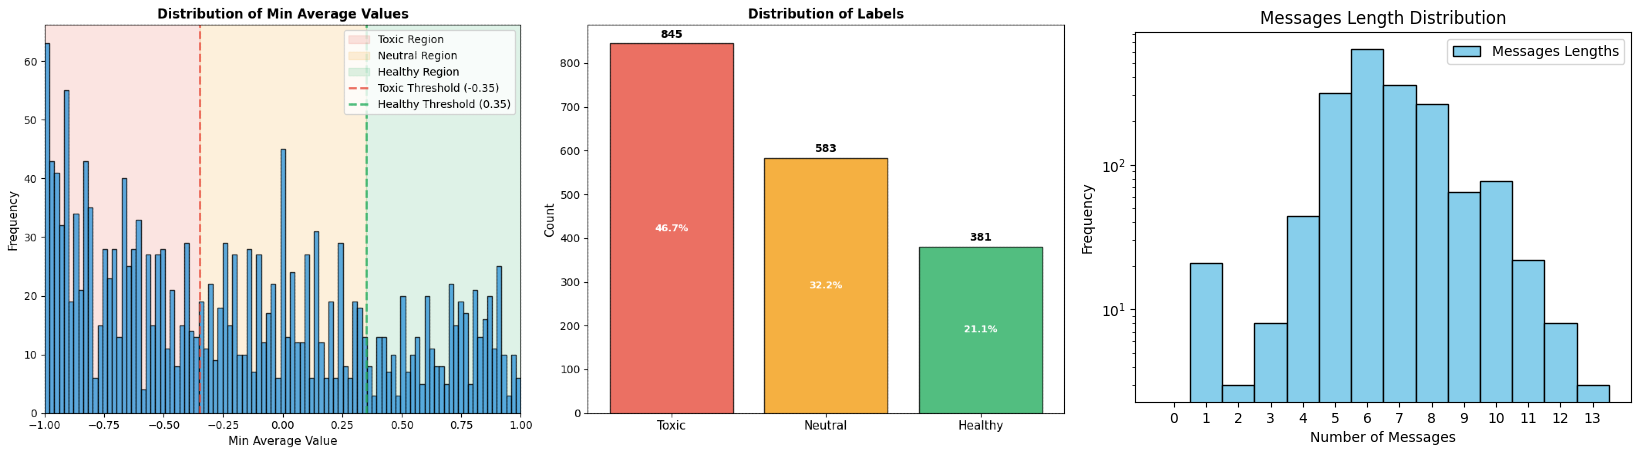
\includegraphics[width=\linewidth]{rsc/multiclass_distributions.png} 
    \caption{Multiclass distribution of the cleaned dataset.}
    \label{fig:multiclass_distribution}
\end{figure*}

\section{Experiments}

For the classification task, we used \texttt{scikit-learn} \textbf{Multinomial Naive Bayes} (NB), \textbf{Logistic Regression} (LR), \textbf{Support Vector Classifier} (SVC), \texttt{Hugging Face Transformers} \textbf{BERT}. For the regression task, we used \texttt{Hugging Face Transformers} \textbf{BERT} model and for explanation the \textbf{BART} model. We used \texttt{dbmdz/bert-base-italian-cased} and \texttt{morenolq/bart-it} checkpoints for BERT and BART respectively since both of them are pre-trained on large Italian corpora. In the multiclass classification task, NB and LR are trained using both a cost-agnostic and a cost-sensitive approach. The cost-sensitive versions employ a custom wrapper that incorporates a predefined cost matrix%
%
% Matrix with square brackets
\[
M =
\begin{bmatrix}
0 & 8 & 16 \\
8 & 0 & 1 \\
16 & 4 & 0 \\
\end{bmatrix}%
\]
%
to minimize the expected misclassification cost during prediction. This is particularly relevant since the costs of different types of misclassifications can vary significantly. Before any training could actually take place, we performed several preprocessing steps to prepare the data for model ingestion. These depends on the model used and are described in the following subsections.

\subsection{Pipelines for \texttt{scikit-learn} Classification Models}

Before model training, the raw text data, which consists of concatenated messages from a single chat, undergoes a multi-stage NLP preprocessing pipeline. This pipeline is designed to prepare data for model ingestion and to reduce feature space dimensionality, normalize the text and anonymize sensitive information. The steps are executed as follows:
\begin{itemize}
    \item \textbf{Tokenization and Linguistic Annotation:} The Italian model from the \texttt{spaCy} library (\texttt{it\_core\_news\_sm}) is utilized for tokenization and linguistic annotation, including Part-of-Speech (POS) tagging and Named Entity Recognition (NER).
    \item \textbf{Anonymization:} To protect user privacy and prevent the models from learning spurious correlations based on specific names or locations, Named Entities corresponding to persons (\texttt{PERSON}), organizations (\texttt{ORG}), and locations (\texttt{LOC}) are identified and replaced with generic placeholders.
    \item \textbf{Part-of-Speech Filtering:} The vocabulary is pruned by retaining only tokens that belong to a whitelist of content-bearing POS tags. This list includes verbs (\texttt{VERB}), adjectives (\texttt{ADJ}), adverbs (\texttt{ADV}), nouns (\texttt{NOUN}), interjections (\texttt{INTJ}), pronouns (\texttt{PRON}), and auxiliary verbs (\texttt{AUX}). This step filters out function words that are less likely to carry semantic weight for the toxicity detection task.
    \item \textbf{Normalizer:} Filtered tokens are normalized using the Italian Snowball Stemmer, provided by the \texttt{nltk} library, or using lemmatization with \texttt{spaCy}. This normalization step reduces different inflections of a word to a common root, thereby consolidating features and reducing sparsity in the feature space. For subsequent sections we will refer to these two pipelines as "\textbf{PosNerLemma-}" and "\textbf{PosNerStem-}" depending on the normalization method used.
\end{itemize}
The output of this preprocessing pipeline is a list of stemmed tokens for each chat document, which serves as the input for the subsequent vectorization stage. Two \texttt{scikit-learn} vectorization methods are explored: \texttt{CountVectorizer} for the Naive Bayes models and \texttt{TfidfVectorizer} for Logistic Regression and SVC.

\subsection{Pipelines for BERT Models}

For BERT models used in \textbf{classification} tasks, we explored two main preprocessing pipelines to structure the chat conversations for model ingestion. The first, simpler pipeline (identified as \textbf{BERT} in subsequent sections) concatenates all messages of a conversation into a single string, separated by newline characters. The special classification token `[CLS]` is prepended to the beginning of the entire chat string. The resulting text is then fed into the BERT tokenizer. The second, more advanced pipeline (identified as \textbf{BERT-ST} in subsequent sections) aims to provide the model with explicit information about speaker turns. In addition to the steps from the simple pipeline, messages from different users are then separated by the special `[SEP]` token and individual tokens are mapped to their respective user via token-type IDs (e.g., 0 for User A and 1 for User B). This creates a structured input like `[CLS] User A: message 1 [SEP] User B: message 2 [SEP] User A: message 3 [SEP] ...`, which helps the model distinguish between speakers and better understand the conversational dynamics.

For the \textbf{regression} task, where the model predicts a toxicity score for each message, a specific preprocessing strategy is employed to create one training sample per message. For each message designated as the "target" within a chat, the entire conversation is formatted as a single input sequence. The target message is uniquely identified by wrapping it with `[SEP]` tokens (e.g., `[SEP] User A: target message [SEP]`), while all other context messages in the chat are included as plain text. The special `[CLS]` token is prepended to the entire sequence. This structure allows the model to focus on a specific message while retaining the full conversational context. To further enhance the model's contextual understanding, we explored two pipelines for the regression task. The first (identified as \textbf{BERT-M} in subsequent sections) uses token-type IDs to distinguish the target message from the context: tokens belonging to the target message are assigned ID 1 (including the `[CLS]` and `[SEP]` tokens), and all other tokens are assigned ID 0. The second (identified as \textbf{BERT-MU} in subsequent sections), more complex "role-aware" pipeline, in addition to token-type IDs, incorporates custom user-type embeddings. In this setup, each speaker in the conversation is assigned a unique integer ID (e.g., 0 for User A, 1 for User B). These IDs are used to create an additional input tensor, `user\_type\_ids`, which is passed to a modified BERT architecture. This allows the model to learn distinct embeddings for each speaker, which are then added to the standard token and positional embeddings. This modification enables the model to better capture speaker-specific contributions to toxicity and understand the interactional dynamics of the dialogue.

\section{Models Training and Evaluation Protocol}

To obtain an unbiased estimate of model performance while simultaneously optimizing hyperparameters, a \textbf{nested cross-validation} protocol is employed. This approach separates the processes of model selection (hyperparameter tuning) and performance evaluation, mitigating the risk of optimistic performance bias. The protocol is structured with an \textbf{outer 5-fold} cross-validation for \textbf{performance estimation} and an \textbf{inner 3-fold} \texttt{GridSearchCV} cross-validation for \textbf{hyperparameter tuning}. Both loops use a \texttt{GroupKFold} strategy to ensure that all chats from a single couple are contained within the same fold, preventing data leakage at the couple level. This is crucial for maintaining the integrity of the evaluation, as conversations involving the same couple may share contextual and relational dynamics that could otherwise lead to overfitting. Since training BERT models is computationally intensive, we do not perform hyperparameter tuning for them; instead, we fixed carefully chosen hyperparameters and we only used the outer loop for performance evaluation in order to allow comparisons with classical models.

The performance of each classification model is evaluated using a comprehensive set of metrics including accuracy, per class \textbf{precision}, \textbf{recall} and \textbf{F1-score} (all of them \textbf{macro} and \textbf{weighted averaged}), and total \textbf{misclassification cost} (only in the multiclass task). The weighted F1-score is particularly emphasized as it accounts for class imbalance by weighting each class's F1-score by its support (the number of true instances for each class).

The performance of each regression model is evaluated using \textbf{Mean Absolute Error} (MAE), \textbf{Mean Squared Error} (MSE), \textbf{Root MSE} (R-MSE) and \textbf{correlation coefficient} between predicted and true scores. We have also chosen to report metrics relative to a naive baseline that always predicts the mean toxicity score of the training set (\textbf{MAE-r}, \textbf{MSE-r}, \textbf{R-MSE-r}). This provides a more interpretable measure of model performance in relation to a simple heuristic. To compare fine-grained regression performances with the more coarse-grained classification ones, we also derived the preceding \textbf{classification metrics} by thresholding the predicted continuous scores into discrete classes applying the same labeling scheme, used during dataset labeling, at both message and chat levels.

In the multiclass classification task, both loops are set to \textbf{minimize misclassification cost} while in the binary one they are set to \textbf{maximize weighted F1-score}, both computed at chat-level. In the BERT regression task, the trainer is set to chose the checkpoint that \textbf{minimizes the misclassification cost} computed at message-level. The main idea behind this choice is to understand how much the more fine-grained regression task can help in the more coarse-grained classification task. By choosing to optimize the misclassification cost at message-level, instead of the one at chat-level, we will be able to assess if, at equal other cross validation conditions, the more fine-grained regression task can lead to better coarse-grained classification performances by computing classification metrics at chat-level and comparing them with the ones obtained by the classification models. This is based on the hypothesis that by focusing on all individual target messages one at a time along with their context, the model can learn more about the toxicity dynamics of an entire chat.

To train the BART model for explanation generation, an initial 80\%-20\% split, grouped by couples, was performed to create the test set of couples. Subsequently, the remaining 80\% of couples was further split (80\%-20\% still grouped by couples) to create the training and validation sets. This resulted in an approximate final distribution of \textbf{64\%} of couples for \textbf{training}, \textbf{16\%} for \textbf{validation}, and \textbf{20\%} for \textbf{testing}. The training and validation sets were used for training multiple epochs and then selecting the best model checkpoint based on validation performance, while the test set was reserved for the final evaluation of the model's ability to generate coherent and contextually relevant explanations.

The quality of the generated explanations is evaluated using a combination of metrics, including \textbf{BLEU}, \textbf{ROUGE} (1, 2 and L), and \textbf{BERTScore} (precision, recall, F1), which measure the overlap between generated explanations and reference explanations in terms of n-grams, longest common subsequences, and semantic similarity, respectively.

The hyperparameters explored during the grid search for the classical models and the fixed hyperparameters for BERT are detailed in Table \ref{tab:hyperparameters}. For the Support Vector Classifier, default parameters were used, and only the vectorizer's hyperparameters were tuned.

\begin{table}[h]
\centering
\small
\caption{Hyperparameters explored for vectorizers and models.}
\label{tab:hyperparameters}
\resizebox{\linewidth}{!}{%
\begin{tabular}{lll}
\hline
\textbf{Component} & \textbf{Hyperparameter} & \textbf{Values} \\
\hline
\texttt{Count/Tfidf} & \texttt{ngram\_range} & (1, 1), (1, 2), (1, 3) \\
\texttt{Vectorizer} & \texttt{min\_df} & 3, 8, 20 \\
& \texttt{max\_df} & 0.9, 0.95, 0.99 \\
\hline
Multinomial NB & \texttt{alpha} & 0.1, 0.5, 1.0, 2.0 \\
\hline
Logistic Regression & \texttt{C} & 0.1, 1.0, 10.0 \\
& \texttt{max\_iter} & 1000, 2000 \\
\hline
BERT & n. Max. Epochs & 20 \\
& Learning Rate & 3e-5 \\
& Batch Size & 32 \\
& Grad. Accum. Steps & 4 \\
& Weight Decay & 0.001 \\
& Warmup Percentage & 0.1 \\
& Early Stopping & Patience: 4 \\
& LR Scheduler & Reduce on Plateau \\
& (Factor: 0.5, & Patience: 2) \\
\hline
BART & n. Max. Epochs & 20 \\
& Learning Rate & 3e-5 \\
& Batch Size & 4 \\
& Grad. Accum. Steps & 8 \\
& Weight Decay & 0.01 \\
& Warmup Percentage & 0.1 \\
& LR Scheduler & Linear with Warmup \\
\hline
\end{tabular}%
}
\end{table}

\subsection{Statistical Analyses of Model Performances}

To ensure the robustness and reliability of our findings, we conducted a series of statistical analyses on the model performance metrics obtained from the nested cross-validation protocol. For each evaluation metric, we first computed the \textbf{mean} and \textbf{standard deviation} across the five outer folds of the cross-validation. This provides a summary of the model's performance and its variability. Then we also computed the \textbf{95\% confidence intervals} (CIs) for each metric using the t-distribution. The CIs offer insights into the precision of our performance estimates and help assess the statistical significance of differences between models.

To determine whether the performance differences between the various model pipelines are statistically significant, a paired statistical test is conducted. The performance of each model configuration is compared against every other configuration using a \textbf{paired t-test}. This test is appropriate because all models are evaluated on the identical set of cross-validation folds created by the outer loop of the nested CV protocol. The comparison is based on the list of weighted F1-scores obtained from each of the five outer folds, allowing for a rigorous assessment of model superiority.

\section{Results}

This section presents the empirical results of our experiments, organized by task: chat-level classification (multiclass and binary), message-level regression, and explanation generation. We analyze the performance of various models and preprocessing pipelines, highlighting key findings and statistical comparisons.

\paragraph{Chat-Level Toxicity Classification}

The performance of all models on the chat-level classification tasks is detailed in Tables \ref{tab:model_comparison} (multiclass) and \ref{tab:model_comparison_regression} (binary).

% Multiclass Classification:
In the \textbf{three-class} (toxic, neutral, healthy) setting, the top-performing models achieve a weighted F1-score of approximately from 0.76 to 0.78. As detailed in Table \ref{tab:model_comparison}, the classic Logistic Regression and SVC models perform on par with both standard BERT classification models. The paired t-tests, visualized in Figure \ref{fig:multiclass_statistical_tests}, confirm that there is no statistically significant performance difference between these top models. This suggests that with robust feature engineering, traditional models can remain competitive with transformer-based architectures on this dataset.

Notably, several experimental variations yielded interesting insights. First, the choice between stemming (PosNerStem) and lemmatization (PosNerLemma) had no statistically discernible impact on performance for any of the classic models, with results being identical across metrics. Second, the cost-sensitive (CS) versions of Naive Bayes and Logistic Regression did not outperform their standard counterparts, indicating that the class weighting inherent in the weighted F1-score metric was sufficient to handle the moderate class imbalance. Lastly, the BERT model with explicit speaker-turn separation (BERT-ST) did not show an improvement over the simpler concatenated input format (BERT), suggesting the base model was already capable of capturing the necessary contextual cues from the raw text sequence.

% Binary Classification
As shown in Table \ref{tab:model_comparison_regression}, the binary task (toxic vs. non-toxic) proved to be significantly easier for all models, with top F1-scores reaching 0.87. The SVC model and the BERT models (BERT, BERT-ST, and the regression-derived BERT-M) were the strongest performers. The statistical tests in Figure \ref{fig:binary_statistical_tests} again show that the performance differences among these leading models are not statistically significant.

\paragraph{Message-Level Toxicity Regression}

The results for the message-level regression task, which predicts a continuous toxicity score for each message, are presented in Table \ref{tab:performance_metrics}. Both the standard BERT regression model (BERT-M) and our proposed role-aware variant (BERT-MU) demonstrated a strong ability to capture the nuances of message-level toxicity, achieving a high correlation coefficient of over 0.82 with the ground-truth scores. The low relative error metrics (e.g., R-MAE of ~0.46) indicate a substantial improvement over a naive baseline that predicts the mean score.

Contrary to our hypothesis, the proposed role-aware architecture with user-type embeddings (BERT-MU) did not yield a substantial performance improvement over the simpler BERT-M model. In fact, BERT-M slightly outperforms BERT-MU across all regression metrics, suggesting that the token-type IDs used to distinguish the target message from its context were sufficient for the model to learn the required dynamics without explicit user embeddings.

\paragraph{Relating Regression and Classification Tasks}

A key objective of our study was to investigate whether a fine-grained regression model could improve performance on the coarser classification task. By aggregating the predicted message-level scores to the chat level, we evaluated the regression models using classification metrics. The results loosely support this hypothesis. As seen in Table \ref{tab:model_comparison}, the regression-based BERT-M model achieves a chat-level weighted F1-score of 0.78 in the multiclass setting, slightly outperforming the direct BERT classifier (0.77) and achieving the lowest misclassification cost (0.10) alongside it. However, the differences in performance are not statistically significant compared to the other BERT variants. BERT-M statistically outperforms only LR and NB variants. In the binary task, the regression-derived BERT-M model performs identically to the best direct classifier (0.87 F1-score), further demonstrating the loosely confirmation of our hypothesis.

\paragraph{Explanation Generation}

The performance of the BART model on the abstractive explanation generation task is summarized in Table \ref{tab:test_metrics}. The model achieved strong results, particularly in semantic similarity. The high BERTScore F1 of 0.77 indicates that the generated explanations are semantically well-aligned with the ground-truth rationales, even when the exact wording differs. The ROUGE-1 score of 0.56 suggests good lexical overlap in terms of key unigrams. As expected for an abstractive task with high linguistic variability, the n-gram-based ROUGE-2 (0.21) and BLEU (0.20) scores are lower but still indicate reasonable fluency and content preservation. Overall, these results confirm the model's capability to produce a bit of coherent and contextually relevant human-readable explanations for its toxicity assessments. Performances are surely promising, but there is still room for improvement, especially in generating more detailed and coherent rationales.

\begin{table}[htbp]
    \centering
    \caption{Performance metrics for the BART explanation generation model.}
    \label{tab:test_metrics}
        \begin{tabular}{lr}
        \hline
        \textbf{Metric} & \textbf{Value} \\
        \hline
        ROUGE-1 & 0.56 \\
        ROUGE-2 & 0.21 \\
        ROUGE-L & 0.25 \\
        BLEU & 0.20 \\
        BERTScore (Precision) & 0.77 \\
        BERTScore (Recall) & 0.76 \\
        BERTScore (F1) & 0.77 \\
        \hline
    \end{tabular}
\end{table}

\begin{figure}[htbp]
    \centering
    % \resizebox{\columnwidth}{!}{%
        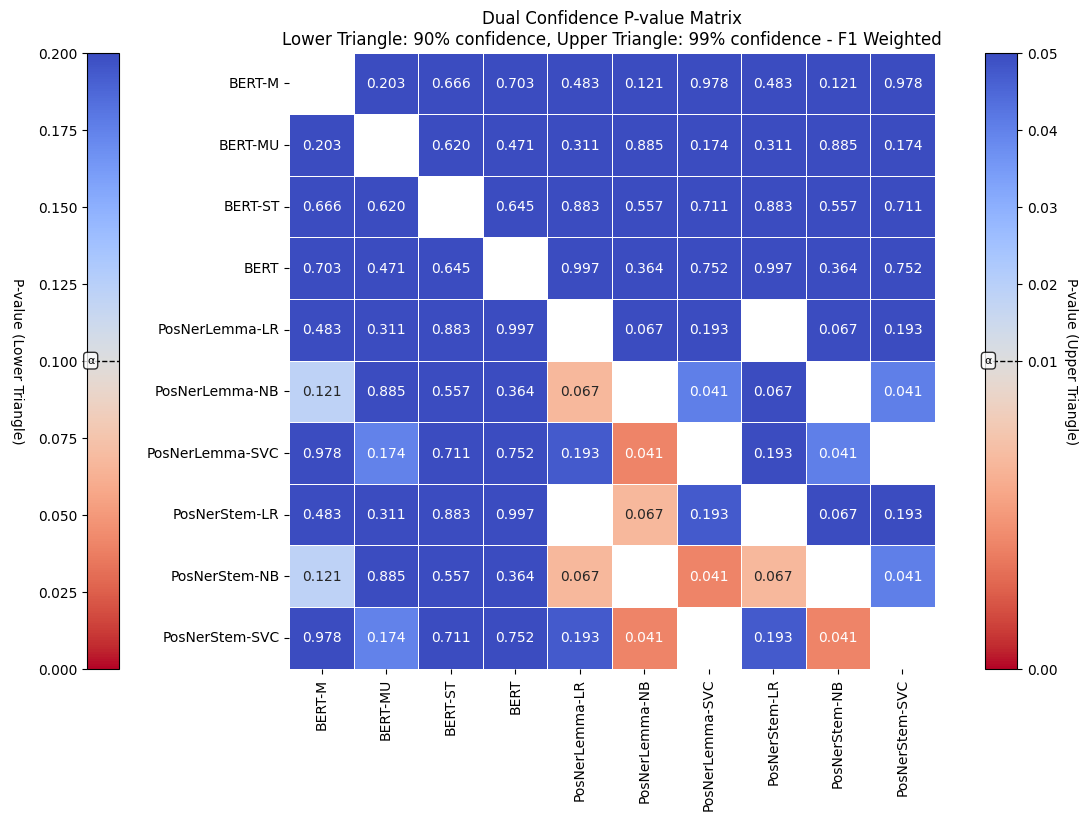
\includegraphics[width=1.0\columnwidth]{rsc/binary_statistical_tests2.png}%
    % }
    \caption{Statistical test results for binary classification performance comparisons between different models or conditions performed on F1-Weighted scores. The lower triangular matrix shows p-values from paired t-tests with a confidence level of 0.90. The upper one shows p-values with a confidence level of 0.99.}
    \label{fig:binary_statistical_tests}
\end{figure}

\begin{figure}[htbp]
    \centering
    % \resizebox{\columnwidth}{!}{%
        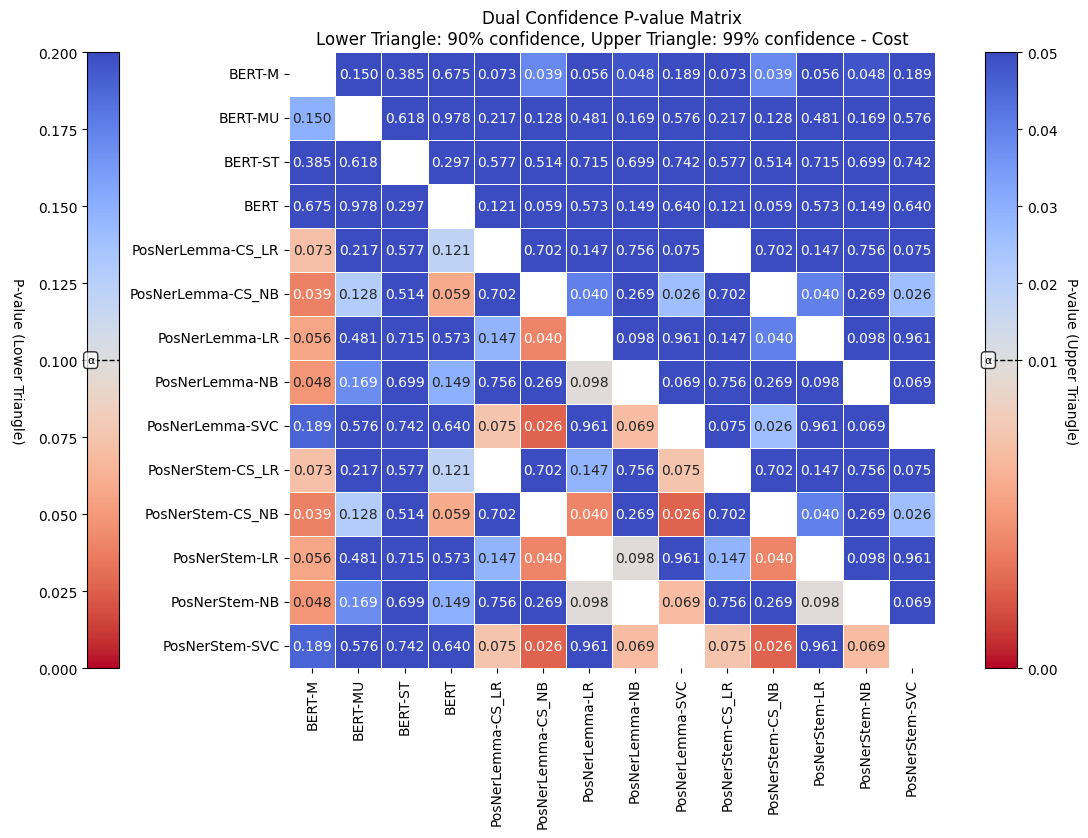
\includegraphics[width=1.0\columnwidth]{rsc/multiclass_statistical_tests2.png}%
    % }
    \caption{Statistical test results for multiclass classification performance comparisons between different models or conditions performed on Cost scores. The lower triangular matrix shows p-values from paired t-tests with a confidence level of 0.90. The upper one shows p-values with a confidence level of 0.99.}
    \label{fig:multiclass_statistical_tests}
\end{figure}

\section{Conclusion and Future Work}

In this paper, we addressed the complex challenge of detecting and explaining toxicity in intimate Italian textual dialogues. We introduced a novel, psychologically-grounded pipeline for generating a rich synthetic dataset, complete with message-level continuous polarity scores and narrative explanations. Our empirical investigation spanned chat-level classification, message-level regression, and abstractive explanation generation, comparing traditional machine learning models with various transformer-based architectures.

A principal and somewhat unexpected finding of this study is the performance plateau observed across a diverse range of models. Both traditional machine learning classifiers, such as Logistic Regression and SVC with robust feature engineering, and advanced transformer-based architectures like BERT achieved statistically indistinguishable peak performances. This convergence suggests that model complexity may not be the primary limiting factor for this task. We hypothesize that this performance ceiling could be attributed to several factors. Firstly, the task of identifying toxicity in intimate conversations is inherently noisy and subjective; what constitutes toxicity can be ambiguous and highly context-dependent, making it difficult for any model to achieve near-perfect accuracy. Secondly, our labeling method, which derives discrete classes by thresholding continuous polarity scores, may introduce fuzzy decision boundaries that challenge all models equally. Finally, the dataset generation pipeline, while systematically designed, may produce data with specific characteristics or latent biases that are learnable up to a certain point by any sufficiently complex model, beyond which further architectural sophistication yields diminishing returns.

Our exploration of a fine-grained regression task proved promising, demonstrating that a BERT model can predict message-level toxicity with high correlation to ground-truth scores. While converting these regression outputs to class labels did not yield a statistically significant improvement over direct classification, it achieved a competitive performance, validating the fine-grained approach. Furthermore, our BART model for explanation generation showed a promising capability for producing semantically relevant rationales, marking a crucial step towards building transparent and trustworthy systems.

Building on these findings, our future work will focus on several key directions aimed at enhancing the robustness and real-world applicability of our approach:

\begin{enumerate}
    \item \textbf{Enhancing Data Generation and Quality Assessment:} We plan to refine our data generation pipeline by incorporating more sophisticated controls and introducing robust quality metrics. This includes developing automated metrics to assess linguistic diversity, psychological plausibility, and annotation consistency. We will explore leveraging multi-agent frameworks, such as crewai, to create a more dynamic and adversarial generation process where one agent generates content while another critiques it, thereby improving the overall quality and realism of the synthetic dataset.

    \item \textbf{Real-World Validation:} A critical next step is to validate the effectiveness of our dataset and the models trained on it. We aim to deploy a public demo in which users can interact with the system and provide feedback on its toxicity assessments and explanations. This will allow us to bridge the "sim-to-real" gap and assess how well our models generalize to the complexities and nuances of authentic human interactions.

    \item \textbf{Multi-Task Learning for Enhanced Explainability:} We will explore a multi-task learning framework by training a single BART-based model to perform both regression (predicting message-level polarity scores) and conditional generation (producing explanations). The hypothesis is that forcing the model to generate a coherent explanation may act as a form of regularization, leading it to learn more robust and generalizable representations of toxic dynamics and hopefully providing better performances on both tasks.

    \item \textbf{Interdisciplinary Collaboration:} To ensure the psychological fidelity and ecological validity of our work, we will deepen our collaboration by including professional psychologists as integral members of the research team. Their expertise will be invaluable not only in refining the persona and chat generation phases but also in the manual validation of annotations and the interpretation of model behaviors, ensuring our technical solutions are grounded in a sound understanding of human psychology and relational dynamics.
\end{enumerate}

All code, models, and the synthetic dataset can be found on the following repo: \url{https://github.com/ashkihotah/cipv-assistant/tree/dev}.

\bibliography{cipv-assistant}

\clearpage

% \appendix
% \section{Performance comparisons between classification and regression modeling approaches}

\begin{table*}[H]
    \centering
    \caption{Performance Comparison Between Models with and without Stemming Preprocessing}
    \label{tab:model_comparison}
    \resizebox{\textwidth}{!}{%
        \begin{tabular}{@{}lcccccc@{}}
            \toprule
            \textbf{Model} & \textbf{Accuracy} & \textbf{Weighted Precision} & \textbf{Weighted Recall} & \textbf{Weighted F1} & \textbf{Cost} \\
            \midrule
            \multicolumn{6}{l}{\textbf{Multiclass Classification Models}} \\
            \midrule
            PosNerStem-CS\_LR & $0.73 \pm 0.03\,[0.69, 0.77]$ & $0.73 \pm 0.03\,[0.68, 0.77]$ & $0.73 \pm 0.03\,[0.69, 0.77]$ & $0.73 \pm 0.03\,[0.68, 0.77]$ & $0.12 \pm 0.02\,[0.09, 0.15]$ \\
            PosNerStem-CS\_NB & $0.74 \pm 0.03\,[0.70, 0.78]$ & $0.75 \pm 0.03\,[0.71, 0.80]$ & $0.74 \pm 0.03\,[0.70, 0.78]$ & $0.75 \pm 0.03\,[0.70, 0.79]$ & $0.12 \pm 0.02\,[0.10, 0.15]$ \\
            PosNerStem-LR & $0.77 \pm 0.02\,[0.74, 0.79]$ & $0.76 \pm 0.02\,[0.73, 0.79]$ & $0.77 \pm 0.02\,[0.74, 0.79]$ & $0.76 \pm 0.02\,[0.73, 0.79]$ & $0.11 \pm 0.01\,[0.09, 0.12]$ \\
            PosNerStem-NB & $0.75 \pm 0.04\,[0.70, 0.80]$ & $0.76 \pm 0.04\,[0.70, 0.81]$ & $0.75 \pm 0.04\,[0.70, 0.80]$ & $0.75 \pm 0.04\,[0.70, 0.80]$ & $0.12 \pm 0.02\,[0.09, 0.15]$ \\
            PosNerStem-SVC & $0.77 \pm 0.02\,[0.73, 0.80]$ & $0.77 \pm 0.03\,[0.73, 0.81]$ & $0.77 \pm 0.02\,[0.73, 0.80]$ & $0.77 \pm 0.03\,[0.73, 0.80]$ & $0.11 \pm 0.01\,[0.09, 0.13]$ \\
            % \midrule
            % \multicolumn{6}{l}{\textbf{Without Stemming (SpacyPosNerPreprocessor)}} \\
            \midrule
            PosNerLemma-CS\_LR & $0.73 \pm 0.03\,[0.69, 0.77]$ & $0.73 \pm 0.03\,[0.68, 0.77]$ & $0.73 \pm 0.03\,[0.69, 0.77]$ & $0.73 \pm 0.03\,[0.68, 0.77]$ & $0.12 \pm 0.02\,[0.09, 0.15]$ \\
            PosNerLemma-CS\_NB & $0.74 \pm 0.03\,[0.70, 0.78]$ & $0.75 \pm 0.03\,[0.71, 0.80]$ & $0.74 \pm 0.03\,[0.70, 0.78]$ & $0.75 \pm 0.03\,[0.70, 0.79]$ & $0.12 \pm 0.02\,[0.10, 0.15]$ \\
            PosNerLemma-LR & $0.77 \pm 0.02\,[0.74, 0.79]$ & $0.76 \pm 0.02\,[0.73, 0.79]$ & $0.77 \pm 0.02\,[0.74, 0.79]$ & $0.76 \pm 0.02\,[0.73, 0.79]$ & $0.11 \pm 0.01\,[0.09, 0.12]$ \\
            PosNerLemma-NB & $0.75 \pm 0.04\,[0.70, 0.80]$ & $0.76 \pm 0.04\,[0.70, 0.81]$ & $0.75 \pm 0.04\,[0.70, 0.80]$ & $0.75 \pm 0.04\,[0.70, 0.80]$ & $0.12 \pm 0.02\,[0.09, 0.15]$ \\
            PosNerLemma-SVC & $0.77 \pm 0.02\,[0.73, 0.80]$ & $0.77 \pm 0.03\,[0.73, 0.81]$ & $0.77 \pm 0.02\,[0.73, 0.80]$ & $0.77 \pm 0.03\,[0.73, 0.80]$ & $0.11 \pm 0.01\,[0.09, 0.13]$ \\
            BERT & $0.77 \pm 0.03\,[0.72, 0.81]$ & $0.77 \pm 0.03\,[0.72, 0.81]$ & $0.77 \pm 0.03\,[0.72, 0.81]$ & $0.77 \pm 0.03\,[0.72, 0.81]$ & $0.10 \pm 0.02\,[0.07, 0.13]$\\
            BERT-ST & $0.76 \pm 0.04\,[0.70, 0.81]$ & $0.76 \pm 0.04\,[0.71, 0.81]$ & $0.76 \pm 0.04\,[0.70, 0.81]$ & $0.76 \pm 0.04\,[0.70, 0.81]$ & $0.11 \pm 0.02\,[0.08, 0.14]$\\
            \midrule
            \multicolumn{6}{l}{\textbf{Regression Models (Chat-Level Classification)}} \\
            \midrule
            BERT-M & $0.78 \pm 0.04\,[0.72, 0.83]$ & $0.79 \pm 0.03\,[0.74, 0.84]$ & $0.78 \pm 0.04\,[0.72, 0.83]$ & $0.78 \pm 0.04\,[0.72, 0.83]$ & $0.10 \pm 0.02\,[0.07, 0.12]$\\
            BERT-MU & $0.77 \pm 0.05\,[0.70, 0.83]$ & $0.78 \pm 0.04\,[0.73, 0.84]$ & $0.77 \pm 0.05\,[0.70, 0.83]$ & $0.77 \pm 0.05\,[0.71, 0.84]$ & $0.10 \pm 0.02\,[0.07, 0.13]$\\
            \midrule
            \multicolumn{6}{l}{\textbf{Regression Models (Message-Level Classification)}} \\
            \midrule
            BERT-M & $0.71 \pm 0.03\,[0.67, 0.76]$ & $0.73 \pm 0.02\,[0.70, 0.75]$ & $0.71 \pm 0.03\,[0.67, 0.76]$ & $0.72 \pm 0.03\,[0.68, 0.76]$ & $0.13 \pm 0.02\,[0.1, 0.15]$\\
            BERT-MU & $0.71 \pm 0.03\,[0.67, 0.75]$ & $0.73 \pm 0.02\,[0.70, 0.76]$ & $0.71 \pm 0.03\,[0.67, 0.75]$ & $0.71 \pm 0.03\,[0.67, 0.75]$ & $0.13 \pm 0.02\,[0.11, 0.15]$\\
            \bottomrule
        \end{tabular}%
    }
\end{table*}

\begin{table*}[H]
    \centering
    \caption{Performance Comparison Between Binary Classification and Regression Models}
    \label{tab:model_comparison_regression}
    % \resizebox{\textwidth}{!}{%
        \begin{tabular}{@{}lcccc@{}}
            \toprule
            \textbf{Model} & \textbf{Accuracy} & \textbf{Weighted Precision} & \textbf{Weighted Recall} & \textbf{Weighted F1} \\
            \midrule
            \multicolumn{5}{l}{\textbf{Binary Classification Models}} \\
            \midrule
            SVC & $0.87 \pm 0.03\,[0.83, 0.91]$ & $0.87 \pm 0.03\,[0.83, 0.91]$ & $0.87 \pm 0.03\,[0.83, 0.91]$ & $0.87 \pm 0.03\,[0.83, 0.91]$ \\
            LR & $0.86 \pm 0.02\,[0.83, 0.90]$ & $0.86 \pm 0.03\,[0.83, 0.90]$ & $0.86 \pm 0.03\,[0.83, 0.90]$ & $0.86 \pm 0.02\,[0.83, 0.90]$ \\
            NB & $0.84 \pm 0.03\,[0.81, 0.88]$ & $0.85 \pm 0.03\,[0.81, 0.88]$ & $0.84 \pm 0.03\,[0.81, 0.88]$ & $0.84 \pm 0.03\,[0.81, 0.88]$ \\
            BERT & $0.86 \pm 0.02\,[0.84, 0.90]$ & $0.87 \pm 0.02\,[0.84, 0.90]$ & $0.87 \pm 0.02\,[0.84, 0.90]$ & $0.87 \pm 0.02\,[0.84, 0.90]$ \\
            BERT-ST & $0.86 \pm 0.02\,[0.82, 0.89]$ & $0.86 \pm 0.02\,[0.83, 0.90]$ & $0.86 \pm 0.02\,[0.82, 0.89]$ & $0.86 \pm 0.02\,[0.82, 0.89]$ \\
            \midrule
            \multicolumn{5}{l}{\textbf{Regression Models (Chat-level Classification)}} \\
            \midrule
            BERT-M & $0.87 \pm 0.02\,[0.84, 0.90]$ & $0.87 \pm 0.02\,[0.84, 0.90]$ & $0.87 \pm 0.02\,[0.84, 0.90]$ & $0.87 \pm 0.02\,[0.84, 0.90]$ \\
            BERT-MU & $0.86 \pm 0.03\,[0.82, 0.89]$ & $0.86 \pm 0.02\,[0.83, 0.90]$ & $0.86 \pm 0.03\,[0.82, 0.89]$ & $0.86 \pm 0.03\,[0.82, 0.89]$ \\
            \midrule
            \multicolumn{5}{l}{\textbf{Regression Models (Message-Level Classification)}} \\
            \midrule
            BERT-M & $0.84 \pm 0.02\,[0.82, 0.87]$ & $0.84 \pm 0.02\,[0.82, 0.87]$ & $0.84 \pm 0.02\,[0.82, 0.87]$ & $0.84 \pm 0.02\,[0.82, 0.86]$ \\
            BERT-MU & $0.84 \pm 0.02\,[0.81, 0.86]$ & $0.84 \pm 0.02\,[0.81, 0.87]$ & $0.84 \pm 0.02\,[0.81, 0.86]$ & $0.83 \pm 0.02\,[0.80, 0.86]$ \\
            \bottomrule
        \end{tabular}%
    % }
\end{table*}

\begin{table*}[H]
    \centering
    \caption{Performance Metrics of Two Models}
    \label{tab:performance_metrics}
    \small % Make the text slightly smaller to fit
    % \resizebox{\textwidth}{!}{%
        \begin{tabular}{lcc}
            \toprule
            \textbf{Metric} & \textbf{BERT-M} & \textbf{BERT-MU} \\
            \midrule
            Mean Squared Error (MSE) & $0.1367 \pm 0.0168 \ [0.1159, 0.1576]$ & $0.1423 \pm 0.0194 \ [0.1182, 0.1664]$ \\
            Mean Absolute Error (MAE) & $0.2656 \pm 0.0216 \ [0.2388, 0.2925]$ & $0.2695 \pm 0.0223 \ [0.2419, 0.2972]$ \\
            Root Mean Squared Error (RMSE) & $0.3692 \pm 0.0225 \ [0.3413, 0.3972]$ & $0.3765 \pm 0.0257 \ [0.3446, 0.4085]$ \\
            Correlation Coefficient & $0.8335 \pm 0.0264 \ [0.8007, 0.8663]$ & $0.8254 \pm 0.0266 \ [0.7923, 0.8584]$ \\
            Relative MSE (R-MSE) & $0.3205 \pm 0.0391 \ [0.2720, 0.3691]$ & $0.3338 \pm 0.0467 \ [0.2758, 0.3918]$ \\
            Relative MAE (R-MAE) & $0.4618 \pm 0.0372 \ [0.4156, 0.5080]$ & $0.4687 \pm 0.0390 \ [0.4203, 0.5171]$ \\
            Relative RMSE (R-RMSE) & $0.5653 \pm 0.0342 \ [0.5229, 0.6078]$ & $0.5766 \pm 0.0406 \ [0.5261, 0.6270]$ \\
            \bottomrule
        \end{tabular}%
    % }
\end{table*}

% \begin{figure*}[H]
%     \centering
%     \begin{subfigure}{0.4\textwidth}
%         \centering
%         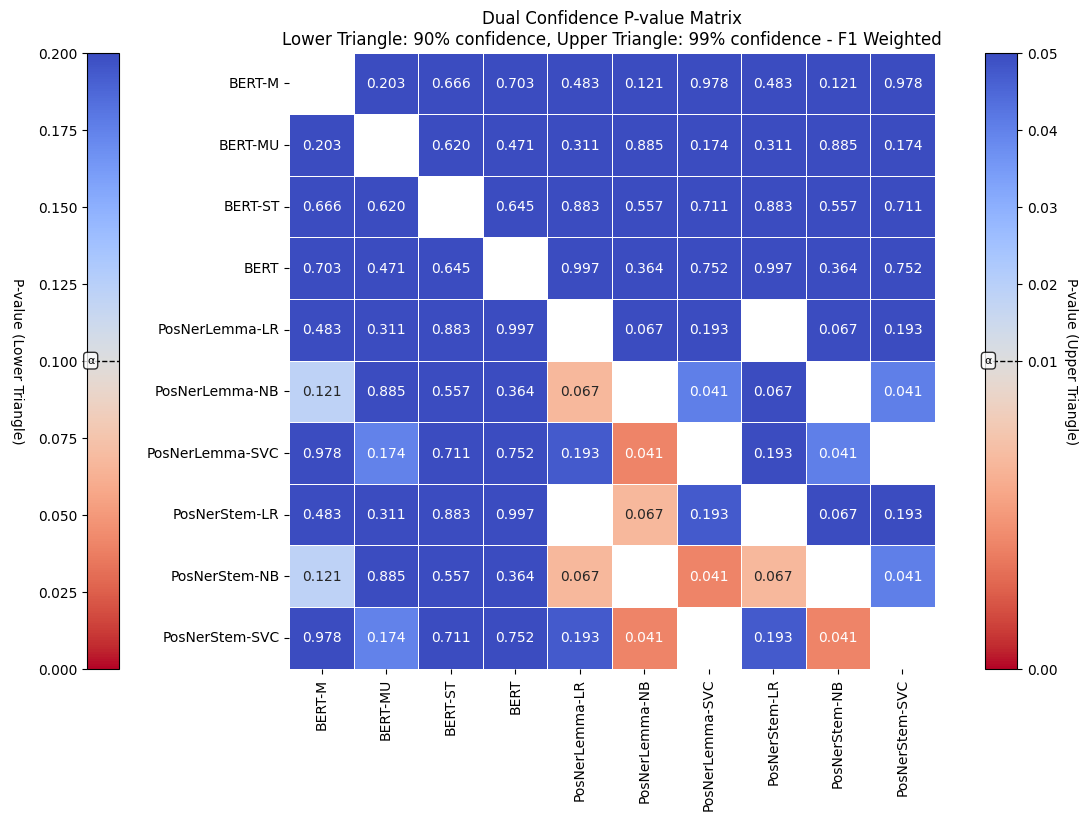
\includegraphics[width=\textwidth]{rsc/binary_statistical_tests2.png}
%         \caption{Binary classification performance comparison}
%         \label{fig:binary_statistical_tests}
%     \end{subfigure}
%     \hfill
%     \begin{subfigure}{0.4\textwidth}
%         \centering
%         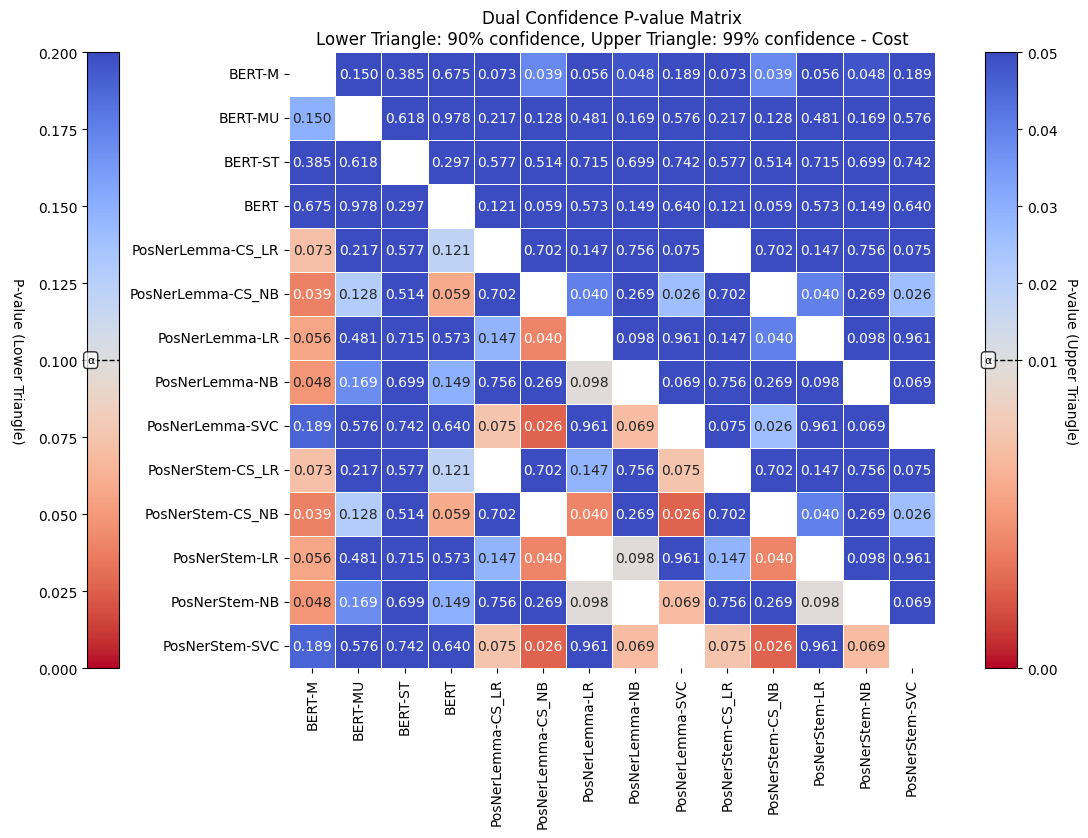
\includegraphics[width=\textwidth]{rsc/multiclass_statistical_tests2.png}
%         \caption{Multiclass classification performance comparison}
%         \label{fig:multiclass_statistical_tests}
%     \end{subfigure}
%     \caption{Statistical test results for classification performance comparison between different models or conditions.}
%     \label{fig:statistical_tests}
% \end{figure*}

\end{document}
